
\section{Methodology}
\begin{comment}
    

\begin{itemize}
    \item Approach/Method Used: Describe the methodology or approach you used for your project (e.g., qualitative, quantitative, experimental, case study).
    \item Tools and Techniques: Detail any tools, software, or technologies you used.
    \item Data Collection: Explain how you gathered data (e.g., surveys, experiments, secondary data).
    \item Data Analysis: Describe the analytical techniques you applied (e.g., statistical analysis, machine learning, content analysis).
\end{itemize}


%\hl{\subsection{Approach}}

%This study extends prior work such as \textcite{joshi2020forecasting}, who employed a single LSTM architecture to forecast the 10-year minus 3-month Treasury yield spread. While Joshi’s application of LSTM demonstrates the potential of deep learning models in economic time series forecasting, it is limited in architectural variation and model tuning. In contrast, this study explores \textbf{multiple LSTM configurations}, including both shallow and stacked architectures, to assess model sensitivity and improve generalization. Additionally, whereas Joshi’s approach focused primarily on the yield spread as a univariate forecasting target, this study integrates the LSTM models into a broader classification framework aimed at directly predicting recession probabilities. This allows for a more practical and policy-relevant application of deep learning in macro-financial forecasting.

% JC

\subsection{Data Collection}

This study utilized quantitative financial data obtained from the Federal Reserve Bank of St. Louis (FRED) database, specifically the 10-year Treasury Yield (GS10), 2-year Treasury Yield (DGS2), and 3-month Treasury Yield (DGS3MO). 

To delineate recessionary periods, official recession dates, defined as the period from peak to trough, were acquired \hl{(from Wikipedia)}, consistent with the National Bureau of Economic Research (NBER) framework. 

\subsection{Tools and Techniques}

Computational analysis for this research was primarily performed using Python within a Jupyter Notebook environment.


\subsection{Data Analysis}

Initial data preprocessing involved the application of forward-fill imputation to address missing values. This approach was chosen to preserve data integrity and ensure the continuity of time series features without introducing spurious noise. 



\hl{Subsequently, the preprocessed dataset was utilized to create 2 features and 1 label column, 2 features were created from the initial datasets, the features are; GS10 - DGS2 and GS10 - DGS3MO}


%Subsequently, the preprocessed dataset was utilized for training a diverse set of predictive models, encompassing both classical econometric approaches—such as Linear Regression and Logistic Regression—and advanced machine learning algorithms, including Long Short-Term Memory (LSTM) networks, Balanced Random Forest, XGBoost, and Easy Ensemble Classifier. 

Subsequently, the features and label dataset was utilized for training a diverse set of predictive models, 

encompassing both classical econometric approaches—such as Logistic Regression—and advanced machine learning algorithms, such as XGBoost, Balanced Random Forest, Easy Ensemble and various configurations for LSTM.

Following model implementation, a comprehensive analysis of the results was conducted to evaluate predictive performance and generate future recession forecasts. The specific methodologies, model architectures, and experimental designs employed in this study will be elaborated in the subsequent sections of this report.


\end{comment}


%#########################################################



%\section{Methodology}

\begin{comment}
\begin{itemize}
    %\item Approach/Method Used: Describe the methodology or approach you used for your project (e.g., qualitative, quantitative, experimental, case study).
    \item Tools and Techniques: Detail any tools, software, or technologies you used.
    \item Data Collection: Explain how you gathered data (e.g., surveys, experiments, secondary data).
    \item Data Analysis: Describe the analytical techniques you applied (e.g., statistical analysis, machine learning, content analysis).
\end{itemize}
\end{comment}



%#################################################################




\subsection{Approach}
This study adopts a quantitative and experimental approach to investigate the predictive relationship between yield curve dynamics and U.S. recessionary periods. The methodology is grounded in empirical modeling and computational experimentation, aiming to quantify the extent to which various term spreads and machine learning models can accurately forecast recessions.

The quantitative aspect is reflected in the use of structured time-series data and statistical indicators derived from Treasury yields, processed to generate explanatory features. The experimental component involves the systematic development, training, and evaluation of multiple predictive models under controlled conditions. These include traditional econometric models and modern machine learning classifiers, all tested on consistent datasets with standardized performance metrics. This dual approach ensures both the analytical rigor of hypothesis-driven modeling and the adaptability of data-driven experimentation.

%By combining theoretical economic constructs (e.g., the term spread as a leading indicator) with empirical testing across multiple algorithms and architectures, this methodology enables a robust evaluation of model performance under real-world forecasting constraints, such as class imbalance and non-linear feature interactions.

\subsection{Data Collection}

This study utilizes secondary quantitative data obtained from publicly available economic datasets. The primary source of financial indicators is the Federal Reserve Bank of St. Louis (FRED), from which three daily time series were extracted: the 10-Year Treasury Constant Maturity Rate (GS10), the 2-Year Treasury Constant Maturity Rate (DGS2), and the 3-Month Treasury Bill Rate (DGS3MO). These yield series were selected due to their widespread use in macro-financial research and their theoretical linkage to expectations about future economic activity.

To identify recessionary periods for labeling, the study uses official dates provided by the 
%National Bureau of Economic Research (NBER) 
\textcite{NBERRecession}, %The recession indicator was encoded as a binary target variable, where each day in the dataset is labeled as either within or outside an NBER-designated recession window. The resulting dataset spans multiple decades and includes both recession and non-recession periods, facilitating robust training and evaluation of predictive models under realistic, imbalanced class distributions.


\subsection{Tools and Techniques}

Computational analysis for this research was conducted using Python3 within a Jupyter Notebook environment. %Python was selected due to its extensive support for data science workflows and its well-established libraries for time-series analysis, statistical modeling, and machine learning.

\begin{comment}
Key libraries used include:
\begin{itemize}
    \item \textbf{pandas} and \textbf{NumPy} for data manipulation and numerical computations;
    \item \textbf{scikit-learn} for classical machine learning models (e.g., Logistic Regression, Random Forest) and preprocessing utilities (e.g., SMOTE, train-test split);
    \item \textbf{xgboost} for gradient boosting classifiers;
    \item \textbf{imbalanced-learn} for handling class imbalance using ensemble methods and synthetic oversampling;
    \item \textbf{TensorFlow} and \textbf{Keras} for building, training, and tuning Long Short-Term Memory (LSTM) networks.
\end{itemize}
\end{comment}

%Model evaluation and visualization were supported by \textbf{matplotlib}, \textbf{seaborn}, and \textbf{scikit-learn}'s built-in metrics and plotting utilities. This combination of tools provided a flexible and reproducible environment for end-to-end experimentation and analysis.

\subsection{Data Analysis}

Initial preprocessing of the time-series data involved using forward-fill to handle missing values. This technique was chosen to maintain temporal continuity without introducing artificial volatility or structural breaks.% By carrying the last observed value forward, the method preserves the integrity of daily observations, especially in financial data that may be missing due to holidays or reporting lags.
Subsequently, two features were engineered from the processed data: the 10-year minus 2-year Treasury spread (GS10--DGS2) and the 10-year minus 3-month Treasury spread (GS10--DGS3MO). %These term spreads serve as leading indicators of recessionary risk and were selected based on their theoretical foundation and empirical track record.
A binary target variable was constructed based on the NBER-designated recession dates, labeling each daily observation as either within (1) or outside (0) a recession period. 

%The resulting dataset was used to train a range of predictive models, including Logistic Regression, XGBoost, Balanced Random Forest, Easy Ensemble, and multiple LSTM configurations.

%To address class imbalance—given the relative rarity of recession periods—sampling techniques such as SMOTE (Synthetic Minority Oversampling Technique) and Random UnderSampling were applied. Model performance was evaluated using standard classification metrics, including precision, recall, F1-score, and confusion matrices, to ensure a comprehensive understanding of predictive accuracy and error distribution.
The resulting feature engineered dataset spans \hl{DD-MM-YYYY} to \hl{DD-MM-2025} and includes both recession and non-recession periods, facilitating robust training and evaluation of predictive models under realistic, imbalanced class distributions. \\

\begin{figure}[htbp]
    \centering
    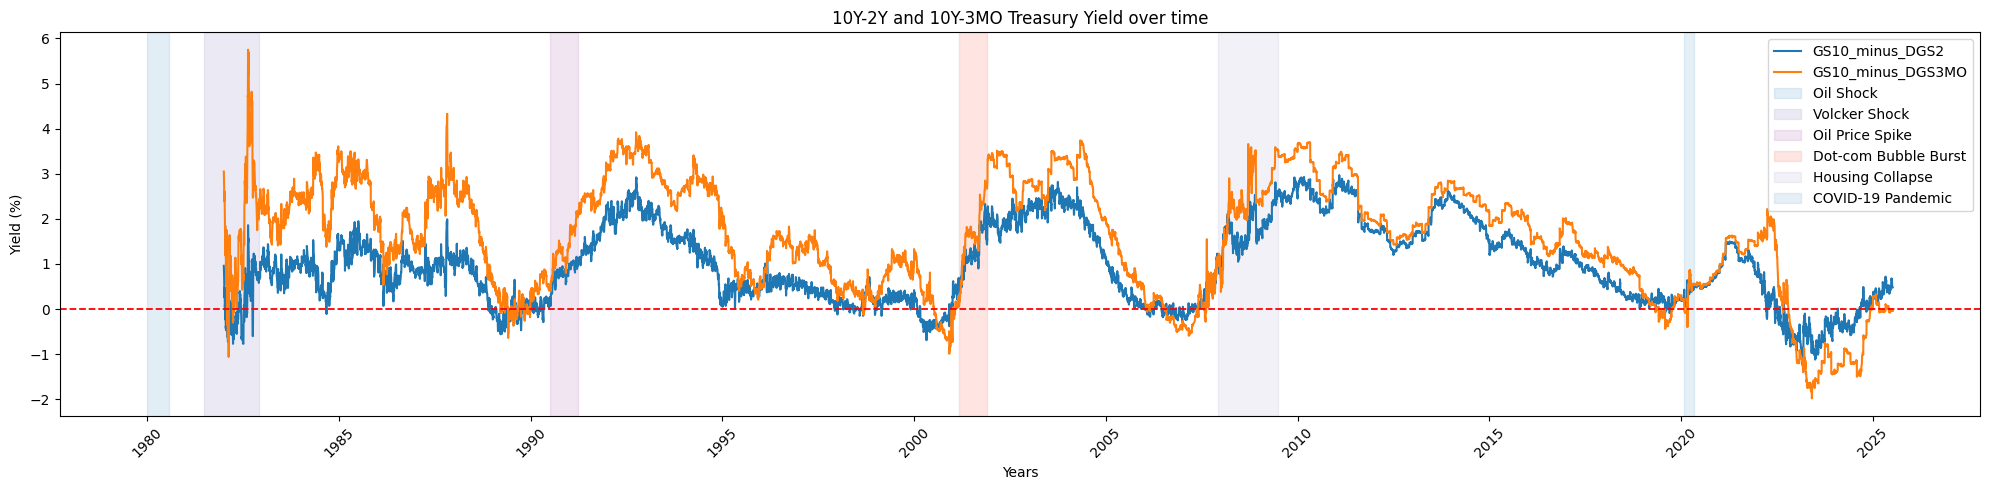
\includegraphics[width=\textwidth-3pt, height=\textheight, keepaspectratio]{Steps/Plots/10Y-2Y and 10Y-3MO Treasury Yield over time.png}
    \caption{10Y-2Y and 10Y-3MO U.S. Treasury Yield Spreads Over Time. %Inversions (when the spread falls below zero) are often viewed as potential indicators of upcoming economic recessions.
    }
    \label{fig:yield-spreads}
\end{figure}

